\documentclass[a4paper]{article}

\usepackage[english]{babel}
\usepackage[utf8]{inputenc}
\usepackage{amsmath}
\usepackage{graphicx}
\usepackage[colorinlistoftodos]{todonotes}
\usepackage{algorithm}
\usepackage{algorithmic}
\usepackage{listings}


\title{COMP90025 Parallel and Multicore Computing \\Project 1b: computing the number of points in the Mandelbrot Set with OpenMPI}

\author{Jiayun He 938828\\Hongming Yi 917352\\The University of Melbourne}

\date{\today}

\begin{document}
\maketitle

\begin{abstract}
The purpose of this project is to parallelise the Mandelbrot Set. We used a few approaches to achieve parallelism and ran tests to tried out. Basically, we divide the node into master node and slave node, the master node read the input and then arrange the task to the rest slave node. When the slave node finish their task, then give the result to the master node.The master node wait until all the node finish the job and add these result together.\end{abstract}

\section{Introduction}
\label{sec:introduction}

The Mandelbrot Set consists of all choices for C(where Z starts at zero and C is a complex number), the condition for choosing C is that giving iterations times,  the Z will never beyond number 2.

\begin{algorithm}
\caption{CountMandelbrotSet}
\begin{algorithmic}
\REQUIRE real\_lower, real\_upper, img\_lower, img\_upper, num, maxiter
\\ count = 0
\\ $real\_step = \frac{real\_upper-real\_lower}{num}$
\\ $img\_step = \frac{img\_upper-img\_lower}{num}$
\FOR{$real = 0\ \TO\ num$}
\FOR{$img = 0\ \TO\ num$}

\STATE $count=Inset(real\_lower+ real\cdot real\_step,  img\_lower+ img\cdot img\_step, maxiter)$

\ENDFOR
\ENDFOR

\end{algorithmic}
\end{algorithm}

The algorithm CountMandelbrotSet firstly read six input, real\_lower and real\_upper are in real axis, img\_lower and img\_upper are in the imaginary axis. The num represents how many parts the real and imaginary axis are divided into.The intersection of the real and imaginary axis represents a possible coordinate of C.The algorithm is to try all the possible situation that C can satisfy the boundary requirement by using two iteration.The first loop is letting value real from zero to num, the second loop is letting value img from zero to num, each times calling the algorithm Inset to check whether C is inset or not. 

\begin{algorithm}
\caption{Inset}
\begin{algorithmic}
\REQUIRE $real, img, maxiter$
\\z\_real = real
\\z\_img = img

\FOR{$iter = 0\ \TO\ maxiter$}
\STATE $z_2\_real = z\_real \cdot z\_real - z\_img $
\STATE $z_2\_img = 2\cdot z\_real \cdot z\_img $
\STATE $z\_real = z_2\_real + real$
\STATE $z\_img = z_2\_img + img$
\IF{$z\_real \cdot z\_real  + z\_img \cdot z\_img > 4$ }
\STATE return 0 
\ENDIF
\ENDFOR
\STATE return 1

\end{algorithmic}
\end{algorithm}

The algorithm Inset is a function that check whether C can satisfy the boundary requirement by using mathematical formula.

\section{Method}
\label{sec:theory}

\subsection{static distribution}
The static distribution evenly distributed the task to each slave node except the last slave node, the process is described in Algorithm3. The partition strategy is to "stride" the area by dividing the range on the real axis.\\Master node use MPI\_Isend method to send tasks to the slave nodes, and different slave node handle distinct tasks. These tasks has different lower and upper bound in real axis and share same range on the imaginary axis.\\
In the main function, according to the rank number, to decide call which type of nodes, if rank equals to zero, then it calls master node, else call slave node. The master will determine partial task and assign value to an array named task, which will be sent to slave node accordingly. 
In the array, task[0] store real\_low,  task[1] store real\_high, task[2] store num. After sending the task to slave node, the master node will wait until all the slave node finish their task.Slave node will report their result by using MPI\_Irecv, finally, the master node add there result together and get the final result.\\
In addition, we add \#pragma omp for in two functions (namely the inset function and the mandelbrotsetCount function). These function both has two loop and each step can be executed individually, so adding the OpenMP Directives can improve the executing speed while retaining the correct answer.

\begin{algorithm}[H]
\begin{algorithmic}
\caption{static divide the task}
\STATE $current\_position = real\_lower$
\STATE $real\_step = (real\_upper-real\_lower)/num$
\STATE $taskCount = worldsize - 1$
\STATE $ taskSize = num / taskCount$
\FOR{$rank = 1\ \TO\ worldsize-1$}
\IF{$rank = nodesNum-1$}
\STATE $task[0] = current\_position$
\STATE $task[1] = real\_upper$
\STATE $task[2] = num - taskSize \cdot (taskCount-1)$
\ELSE 
\STATE $task[0] = current\_position$
\STATE $current\_position += taskSize \cdot real\_step$
\STATE $task[1] = current\_position$
\STATE $task[2] = taskSize$
\ENDIF
\ENDFOR
\end{algorithmic}
\end{algorithm}

\subsection{semi-dynamic distribution}
Unlike static distribution method where taskCount = worldsize - 1, in dynamic distribution method, we add a task\_factor variable. The task\_factor variable indicates the portion of tasks that are not assigned to slave nodes during the initial task distribution. In fact, the static distribution method is a special case with task\_factor equals 1. In this semi-dynamic method, $taskCount = (worldsize - 1)\cdot task\_factor$. By testing different number of task\_factor, we find when task\_factor equals to worldsize, the run time is optimal. And the division of this dynamic method can be found in Algorithm 4.(code applying dynamic distribution called parallel 3). This is a semi-dynamic method because the partitions are predetermined by the size of input and worldsize.

\subsubsection{improved dynamic distribution version}
When doing experiment, we find that if the input num is greater or closer to the value $(worldsize - 1)\cdot task\_factor$, running the dynamic distribution program will result a error output. So in this method, we combine the static distribution method and semi-dynamic distribution method.(in experiment, this version code called parallel 4)
The procedure is following:

\begin{lstlisting}
if((worldsize-1)*TASK_FACTOR < num/2){
        if(myrank == 0) master();
        else slave();
        MPI_Finalize();
}
else{
    if(myrank == 0) parallel2_master();
    else parallel2_slave();
    MPI_Finalize();
}
\end{lstlisting}


\begin{algorithm}[H]
\begin{algorithmic}
\caption{dynamic divide the task}
\STATE //initial distribution
\STATE $current\_position = real\_lower$
\STATE $real\_step = (real\_upper-real\_lower)/num$
\STATE $taskCount = (worldsize - 1)\cdot task\_factor$
\STATE $pending = taskCount$
\STATE $finished = 0$
\STATE $ taskSize = num / taskCount$
\FOR{$rank = 1\ \TO\ worldsize-1$}
\STATE $task[0] = current\_position$
\STATE $current\_position += taskSize \cdot real\_step$
\STATE $task[1] = current\_position$
\STATE $task[2] = taskSize$
\STATE MPI\_Isend(task)
\STATE $pending \gets pending-1$
\ENDFOR
\STATE //when slave node finish their task, they request to master node whether there still has task to do
\WHILE{$finished <= taskCount$}
\STATE MPI\_Irecv from slave node
\STATE $finished \gets finished+1$
\IF{$pending>0$}
\STATE task[0] = current\_position
\IF{$current\_position > real\_upper$}
\STATE $task[1] = real\_upper$
\STATE $task[2] = (num - taskSize \cdot (taskCount-1))$
\STATE $pending \gets pending-1$
\STATE MPI\_Isend(task)
\ELSE
\STATE $task[1] = current\_position$
\STATE $task[2] = taskSize$
\STATE $pending \gets pending-1$
\STATE MPI\_Isend(task)
\ENDIF 
\ENDIF
\ENDWHILE
\end{algorithmic}
\end{algorithm}



\section{Experiment and Results}
To experiment on different algorithms, we tried our program on Spartan, both on the Cloud partition (Only for some experimental tryouts) and the physical partition.
The speedup is calculated by:
\begin{center}
	$S = \frac{T(n)}{P(n)}$
\end{center}
Where p is the number of processors, T(n) is the sequential run time and P(n) is the corresponding parallel run time. 
\subsection{Test on small input}
Most of our experiments are with a relatively small input: -2.0 1.0 -1.0 1.0 1000 10000
\begin{figure}[H]
	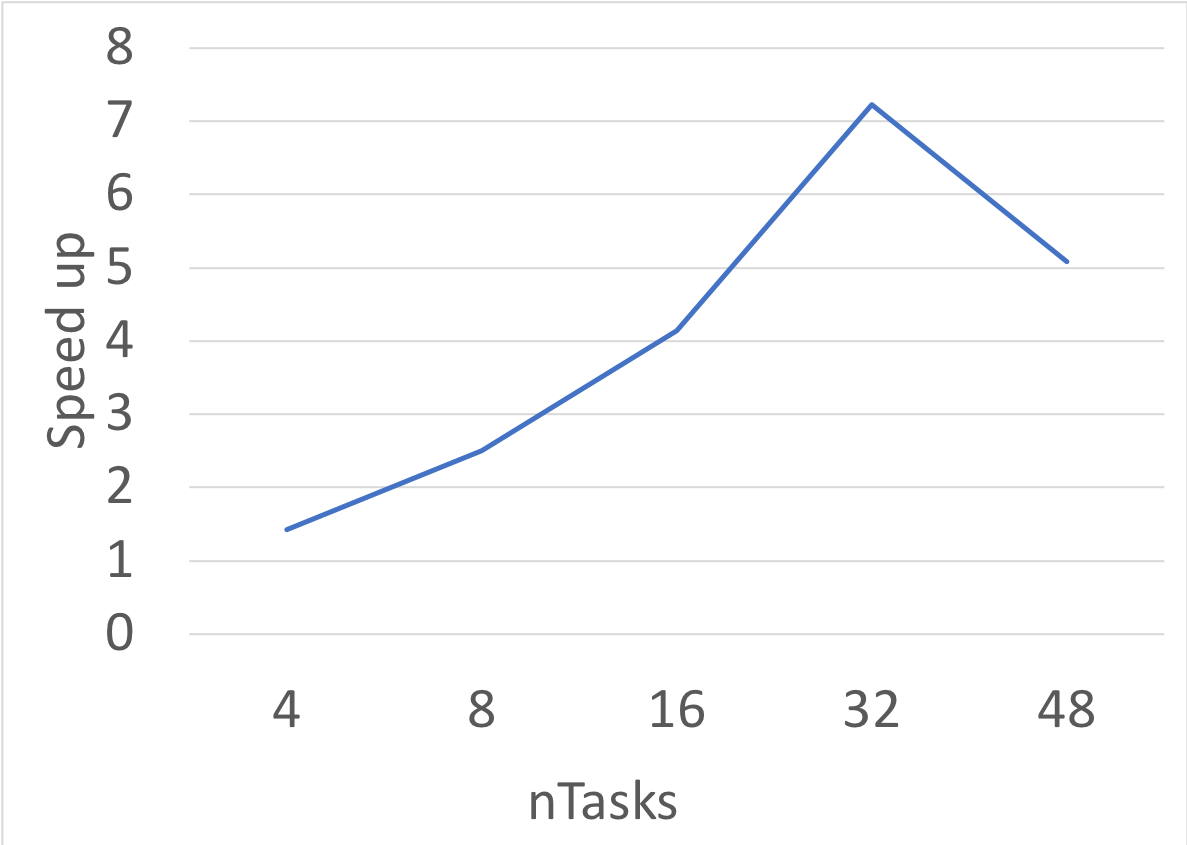
\includegraphics[width=\linewidth]{figure1.png}
	\caption{Speedup in parallel2 (with different nTasks)}
	\label{marker}
\end{figure}
From this figure, we can know that normally, when having more nTasks to calculate, the speedup is increasing, however, when nTasks increase from 32 to 48, the speedup is decreasing. We assumed that it was because some processors are much more heavily loaded than the others, according to the nature of mandelbrot set. We then turned to parallel3, which utilized a semi-dynamic distribution. We experiment different task factors on different number of ntasks (we used the --nodes and --ntasks-per-node options on spartan) to find an optimal value.
\begin{figure}[H]
	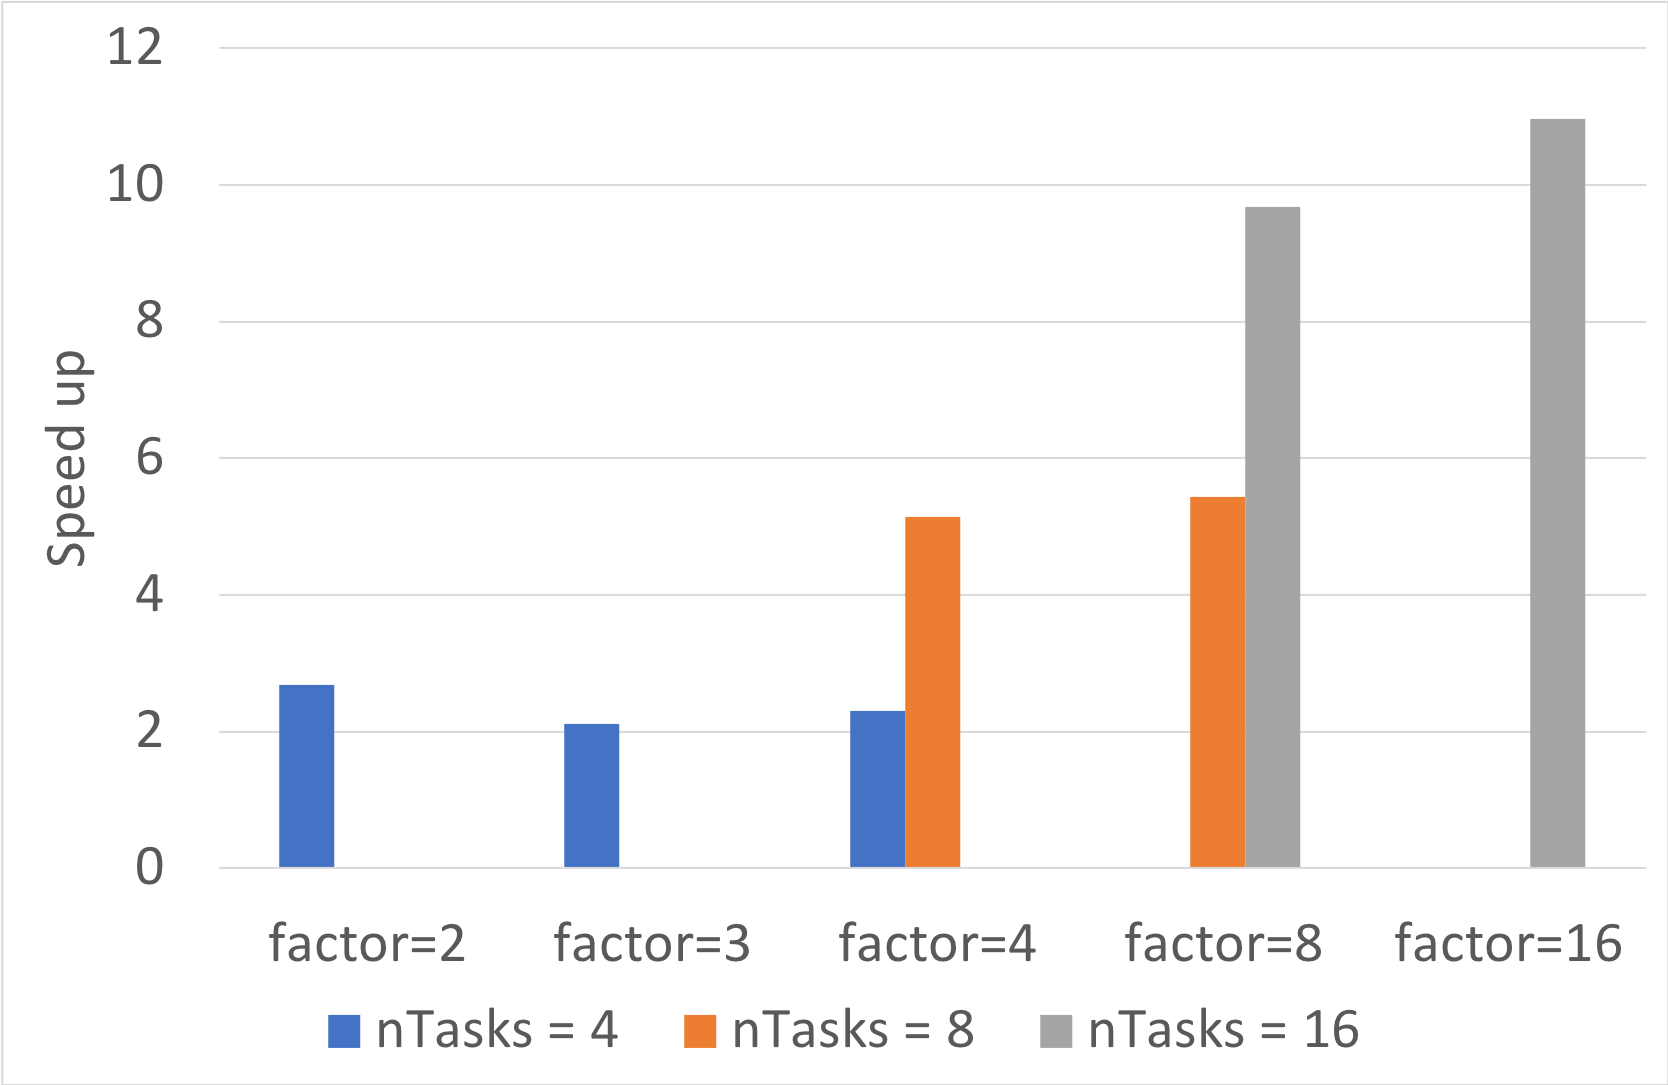
\includegraphics[width=\linewidth]{figure2.png}
	\caption{Speedup with parallel3 (with different nTasks and task factors)}
	\label{marker}
\end{figure}

\begin{figure}[H]
	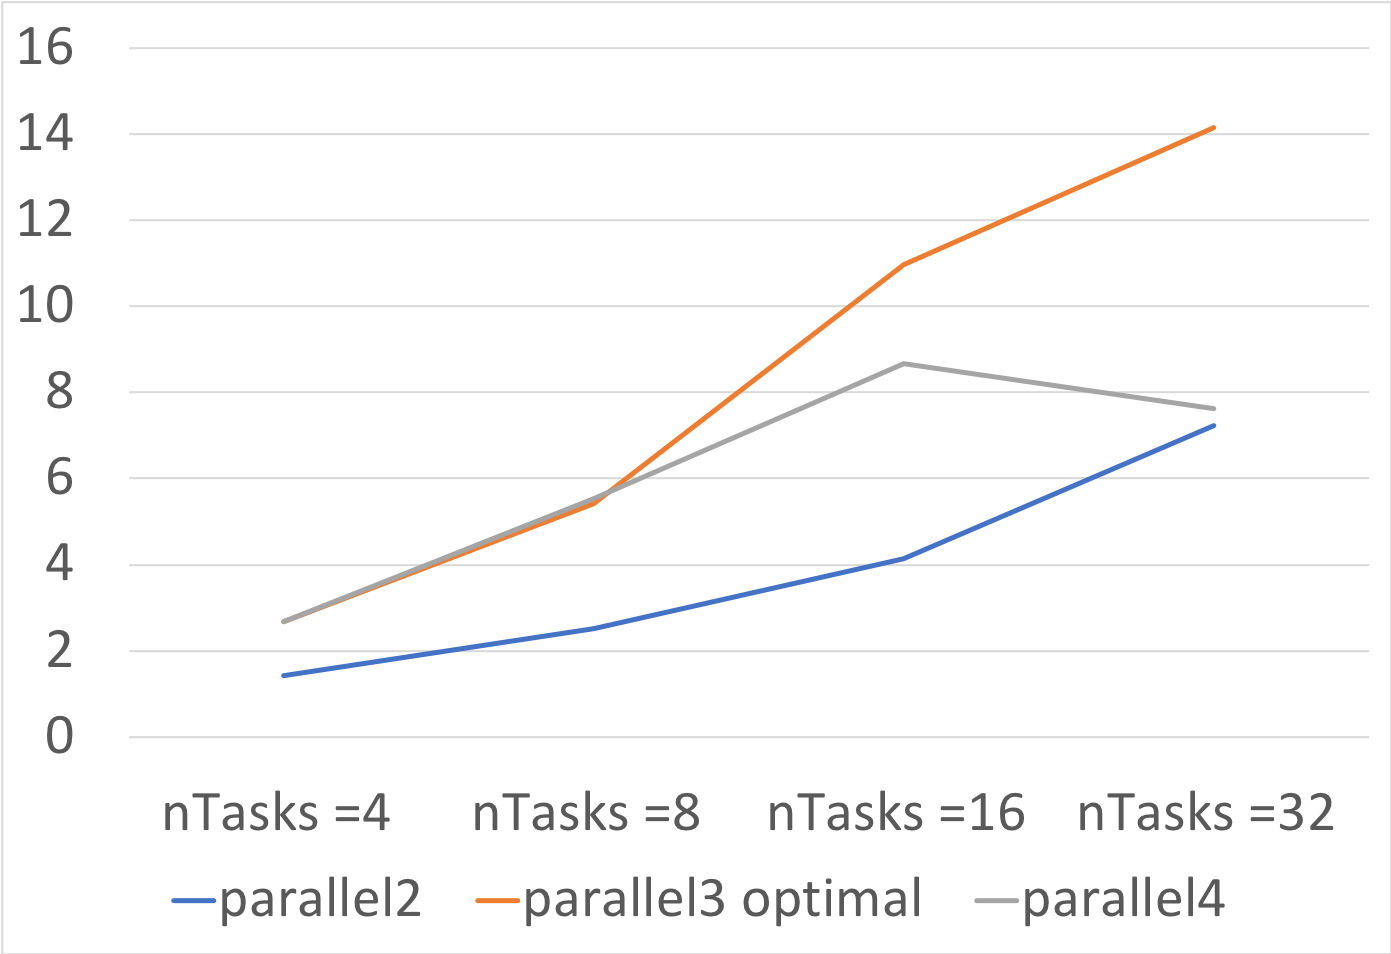
\includegraphics[width=\linewidth]{figure3.png}
	\caption{Speedup from three parallel algorithm}
	\label{marker}
\end{figure}

\subsection{Test on larger input}
We increases the input num to 10000 and compare speedups among different parallel methods. The programs are ran on Spartan's physical partition with 6 nodes (8 ntasks on each node). The parallel3 optimal is parallel3 with a task factor equals to worldsize.
\begin{figure}[H]
	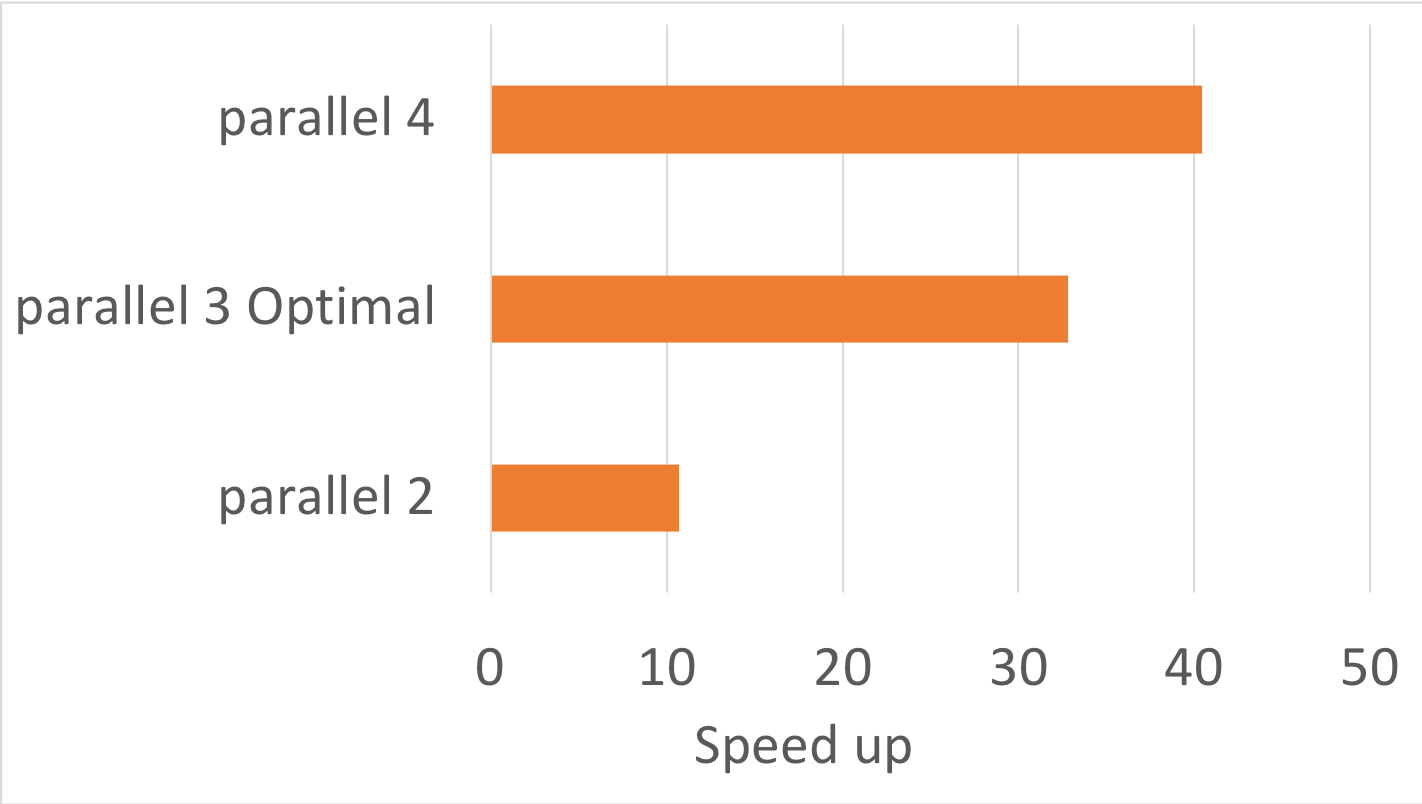
\includegraphics[width=\linewidth]{figure4.png}
	\caption{Speedup from three parallel algorithm on big num(nTasks = 48)}
	\label{marker}
\end{figure}
\noindent Figure 2 implies that different factors result different speedup when the nTasks are the same. From Figure 3, it seems that the optimal of parallel 3 has best speedup, however in Figure 4, when the input number becomes bigger, the parallel4 has the top speedup.

\begin{thebibliography}{9}
\bibitem{nano3}
Charousset, Dominik, Thomas C. Schmidt, Raphael Hiesgen, and Matthias Wählisch. "Native actors: a scalable software platform for distributed, heterogeneous environments." In Proceedings of the 2013 workshop on Programming based on actors, agents, and decentralized control, pp. 87-96. ACM, 2013.

\bibitem{nano3}
Mandelbrot Set problem\\
http://wili.cc/blog/mandelbrot-mpi.html
\end{thebibliography}


\end{document}
